% Options for packages loaded elsewhere
% Options for packages loaded elsewhere
\PassOptionsToPackage{unicode}{hyperref}
\PassOptionsToPackage{hyphens}{url}
\PassOptionsToPackage{dvipsnames,svgnames,x11names}{xcolor}
%
\documentclass[
  russian,
  letterpaper,
  DIV=11,
  numbers=noendperiod]{scrartcl}
\usepackage{xcolor}
\usepackage{amsmath,amssymb}
\setcounter{secnumdepth}{5}
\usepackage{iftex}
\ifPDFTeX
  \usepackage[T1]{fontenc}
  \usepackage[utf8]{inputenc}
  \usepackage{textcomp} % provide euro and other symbols
\else % if luatex or xetex
  \usepackage{unicode-math} % this also loads fontspec
  \defaultfontfeatures{Scale=MatchLowercase}
  \defaultfontfeatures[\rmfamily]{Ligatures=TeX,Scale=1}
\fi
\usepackage{lmodern}
\ifPDFTeX\else
  % xetex/luatex font selection
\fi
% Use upquote if available, for straight quotes in verbatim environments
\IfFileExists{upquote.sty}{\usepackage{upquote}}{}
\IfFileExists{microtype.sty}{% use microtype if available
  \usepackage[]{microtype}
  \UseMicrotypeSet[protrusion]{basicmath} % disable protrusion for tt fonts
}{}
\makeatletter
\@ifundefined{KOMAClassName}{% if non-KOMA class
  \IfFileExists{parskip.sty}{%
    \usepackage{parskip}
  }{% else
    \setlength{\parindent}{0pt}
    \setlength{\parskip}{6pt plus 2pt minus 1pt}}
}{% if KOMA class
  \KOMAoptions{parskip=half}}
\makeatother
% Make \paragraph and \subparagraph free-standing
\makeatletter
\ifx\paragraph\undefined\else
  \let\oldparagraph\paragraph
  \renewcommand{\paragraph}{
    \@ifstar
      \xxxParagraphStar
      \xxxParagraphNoStar
  }
  \newcommand{\xxxParagraphStar}[1]{\oldparagraph*{#1}\mbox{}}
  \newcommand{\xxxParagraphNoStar}[1]{\oldparagraph{#1}\mbox{}}
\fi
\ifx\subparagraph\undefined\else
  \let\oldsubparagraph\subparagraph
  \renewcommand{\subparagraph}{
    \@ifstar
      \xxxSubParagraphStar
      \xxxSubParagraphNoStar
  }
  \newcommand{\xxxSubParagraphStar}[1]{\oldsubparagraph*{#1}\mbox{}}
  \newcommand{\xxxSubParagraphNoStar}[1]{\oldsubparagraph{#1}\mbox{}}
\fi
\makeatother

\usepackage{color}
\usepackage{fancyvrb}
\newcommand{\VerbBar}{|}
\newcommand{\VERB}{\Verb[commandchars=\\\{\}]}
\DefineVerbatimEnvironment{Highlighting}{Verbatim}{commandchars=\\\{\}}
% Add ',fontsize=\small' for more characters per line
\usepackage{framed}
\definecolor{shadecolor}{RGB}{241,243,245}
\newenvironment{Shaded}{\begin{snugshade}}{\end{snugshade}}
\newcommand{\AlertTok}[1]{\textcolor[rgb]{0.68,0.00,0.00}{#1}}
\newcommand{\AnnotationTok}[1]{\textcolor[rgb]{0.37,0.37,0.37}{#1}}
\newcommand{\AttributeTok}[1]{\textcolor[rgb]{0.40,0.45,0.13}{#1}}
\newcommand{\BaseNTok}[1]{\textcolor[rgb]{0.68,0.00,0.00}{#1}}
\newcommand{\BuiltInTok}[1]{\textcolor[rgb]{0.00,0.23,0.31}{#1}}
\newcommand{\CharTok}[1]{\textcolor[rgb]{0.13,0.47,0.30}{#1}}
\newcommand{\CommentTok}[1]{\textcolor[rgb]{0.37,0.37,0.37}{#1}}
\newcommand{\CommentVarTok}[1]{\textcolor[rgb]{0.37,0.37,0.37}{\textit{#1}}}
\newcommand{\ConstantTok}[1]{\textcolor[rgb]{0.56,0.35,0.01}{#1}}
\newcommand{\ControlFlowTok}[1]{\textcolor[rgb]{0.00,0.23,0.31}{\textbf{#1}}}
\newcommand{\DataTypeTok}[1]{\textcolor[rgb]{0.68,0.00,0.00}{#1}}
\newcommand{\DecValTok}[1]{\textcolor[rgb]{0.68,0.00,0.00}{#1}}
\newcommand{\DocumentationTok}[1]{\textcolor[rgb]{0.37,0.37,0.37}{\textit{#1}}}
\newcommand{\ErrorTok}[1]{\textcolor[rgb]{0.68,0.00,0.00}{#1}}
\newcommand{\ExtensionTok}[1]{\textcolor[rgb]{0.00,0.23,0.31}{#1}}
\newcommand{\FloatTok}[1]{\textcolor[rgb]{0.68,0.00,0.00}{#1}}
\newcommand{\FunctionTok}[1]{\textcolor[rgb]{0.28,0.35,0.67}{#1}}
\newcommand{\ImportTok}[1]{\textcolor[rgb]{0.00,0.46,0.62}{#1}}
\newcommand{\InformationTok}[1]{\textcolor[rgb]{0.37,0.37,0.37}{#1}}
\newcommand{\KeywordTok}[1]{\textcolor[rgb]{0.00,0.23,0.31}{\textbf{#1}}}
\newcommand{\NormalTok}[1]{\textcolor[rgb]{0.00,0.23,0.31}{#1}}
\newcommand{\OperatorTok}[1]{\textcolor[rgb]{0.37,0.37,0.37}{#1}}
\newcommand{\OtherTok}[1]{\textcolor[rgb]{0.00,0.23,0.31}{#1}}
\newcommand{\PreprocessorTok}[1]{\textcolor[rgb]{0.68,0.00,0.00}{#1}}
\newcommand{\RegionMarkerTok}[1]{\textcolor[rgb]{0.00,0.23,0.31}{#1}}
\newcommand{\SpecialCharTok}[1]{\textcolor[rgb]{0.37,0.37,0.37}{#1}}
\newcommand{\SpecialStringTok}[1]{\textcolor[rgb]{0.13,0.47,0.30}{#1}}
\newcommand{\StringTok}[1]{\textcolor[rgb]{0.13,0.47,0.30}{#1}}
\newcommand{\VariableTok}[1]{\textcolor[rgb]{0.07,0.07,0.07}{#1}}
\newcommand{\VerbatimStringTok}[1]{\textcolor[rgb]{0.13,0.47,0.30}{#1}}
\newcommand{\WarningTok}[1]{\textcolor[rgb]{0.37,0.37,0.37}{\textit{#1}}}

\usepackage{longtable,booktabs,array}
\usepackage{calc} % for calculating minipage widths
% Correct order of tables after \paragraph or \subparagraph
\usepackage{etoolbox}
\makeatletter
\patchcmd\longtable{\par}{\if@noskipsec\mbox{}\fi\par}{}{}
\makeatother
% Allow footnotes in longtable head/foot
\IfFileExists{footnotehyper.sty}{\usepackage{footnotehyper}}{\usepackage{footnote}}
\makesavenoteenv{longtable}
\usepackage{graphicx}
\makeatletter
\newsavebox\pandoc@box
\newcommand*\pandocbounded[1]{% scales image to fit in text height/width
  \sbox\pandoc@box{#1}%
  \Gscale@div\@tempa{\textheight}{\dimexpr\ht\pandoc@box+\dp\pandoc@box\relax}%
  \Gscale@div\@tempb{\linewidth}{\wd\pandoc@box}%
  \ifdim\@tempb\p@<\@tempa\p@\let\@tempa\@tempb\fi% select the smaller of both
  \ifdim\@tempa\p@<\p@\scalebox{\@tempa}{\usebox\pandoc@box}%
  \else\usebox{\pandoc@box}%
  \fi%
}
% Set default figure placement to htbp
\def\fps@figure{htbp}
\makeatother



\ifLuaTeX
\usepackage[bidi=basic,provide=*]{babel}
\else
\usepackage[bidi=default,provide=*]{babel}
\fi
% get rid of language-specific shorthands (see #6817):
\let\LanguageShortHands\languageshorthands
\def\languageshorthands#1{}


\setlength{\emergencystretch}{3em} % prevent overfull lines

\providecommand{\tightlist}{%
  \setlength{\itemsep}{0pt}\setlength{\parskip}{0pt}}



 


\usepackage{fontspec}

\setsansfont{Palatino Linotype}[
    Path=../files/palatino/,
    Extension = .ttf,
    UprightFont=palatino-Roman,
    BoldFont=palatino-Bold,
    ItalicFont=palatino-Italic,
    BoldItalicFont=palatino-BoldItalic
]
\setmainfont{Palatino Linotype}[
    Path=../files/palatino/,
    Extension = .ttf,
    UprightFont=palatino-Roman,
    BoldFont=palatino-Bold,
    ItalicFont=palatino-Italic,
    BoldItalicFont=palatino-BoldItalic
]

\usepackage[textwidth=0.86\paperwidth, textheight=0.86\paperheight]{geometry}
\usepackage{fancyhdr}
\usepackage{hyperref}
\usepackage{fontawesome5}
\usepackage{graphicx}
\usepackage{amssymb}
\usepackage{amsmath}
\graphicspath{{../files/}}

\newcommand{\R}{\mathbb{R}}

% \pagenumbering{gobble}
\pagestyle{fancy}
\fancyhead{} % clear all header fields
\fancyhead[R]{\href{https://cu25.fmin.xyz}{\faGem[regular]} \hspace{0.04cm} \href{https://github.com/MerkulovDaniil/cu25}{\faGithub} \hspace{0.07cm} \href{https://t.me/fminxyz}{\faTelegram}}
\fancyhead[L]{\href{https://fmin.xyz}{
\includegraphics[height=0.35cm]{logo.pdf}} ~ 
\includegraphics[height=0.35cm]{logo_cu.pdf} \hspace{2pt} \textbf{Оптимизация для всех! ЦУ. 2025}}
\KOMAoption{captions}{tableheading}
\makeatletter
\@ifpackageloaded{tcolorbox}{}{\usepackage[skins,breakable]{tcolorbox}}
\@ifpackageloaded{fontawesome5}{}{\usepackage{fontawesome5}}
\definecolor{quarto-callout-color}{HTML}{909090}
\definecolor{quarto-callout-note-color}{HTML}{0758E5}
\definecolor{quarto-callout-important-color}{HTML}{CC1914}
\definecolor{quarto-callout-warning-color}{HTML}{EB9113}
\definecolor{quarto-callout-tip-color}{HTML}{00A047}
\definecolor{quarto-callout-caution-color}{HTML}{FC5300}
\definecolor{quarto-callout-color-frame}{HTML}{acacac}
\definecolor{quarto-callout-note-color-frame}{HTML}{4582ec}
\definecolor{quarto-callout-important-color-frame}{HTML}{d9534f}
\definecolor{quarto-callout-warning-color-frame}{HTML}{f0ad4e}
\definecolor{quarto-callout-tip-color-frame}{HTML}{02b875}
\definecolor{quarto-callout-caution-color-frame}{HTML}{fd7e14}
\makeatother
\makeatletter
\@ifpackageloaded{caption}{}{\usepackage{caption}}
\AtBeginDocument{%
\ifdefined\contentsname
  \renewcommand*\contentsname{Содержание}
\else
  \newcommand\contentsname{Содержание}
\fi
\ifdefined\listfigurename
  \renewcommand*\listfigurename{Список Иллюстраций}
\else
  \newcommand\listfigurename{Список Иллюстраций}
\fi
\ifdefined\listtablename
  \renewcommand*\listtablename{Список Таблиц}
\else
  \newcommand\listtablename{Список Таблиц}
\fi
\ifdefined\figurename
  \renewcommand*\figurename{Рисунок}
\else
  \newcommand\figurename{Рисунок}
\fi
\ifdefined\tablename
  \renewcommand*\tablename{Таблица}
\else
  \newcommand\tablename{Таблица}
\fi
}
\@ifpackageloaded{float}{}{\usepackage{float}}
\floatstyle{ruled}
\@ifundefined{c@chapter}{\newfloat{codelisting}{h}{lop}}{\newfloat{codelisting}{h}{lop}[chapter]}
\floatname{codelisting}{Список}
\newcommand*\listoflistings{\listof{codelisting}{Список Каталогов}}
\makeatother
\makeatletter
\makeatother
\makeatletter
\@ifpackageloaded{caption}{}{\usepackage{caption}}
\@ifpackageloaded{subcaption}{}{\usepackage{subcaption}}
\makeatother
\usepackage{bookmark}
\IfFileExists{xurl.sty}{\usepackage{xurl}}{} % add URL line breaks if available
\urlstyle{same}
\hypersetup{
  pdftitle={Задача линейного программирования},
  pdfauthor={Даня Меркулов},
  pdflang={ru},
  colorlinks=true,
  linkcolor={blue},
  filecolor={Maroon},
  citecolor={Blue},
  urlcolor={Blue},
  pdfcreator={LaTeX via pandoc}}


\title{Задача линейного программирования}
\author{Даня Меркулов}
\date{}
\begin{document}
\maketitle


\section{Примеры задач линейного
программирования}\label{ux43fux440ux438ux43cux435ux440ux44b-ux437ux430ux434ux430ux447-ux43bux438ux43dux435ux439ux43dux43eux433ux43e-ux43fux440ux43eux433ux440ux430ux43cux43cux438ux440ux43eux432ux430ux43dux438ux44f}

\subsection{Что такое линейное
программирование?}\label{ux447ux442ux43e-ux442ux430ux43aux43eux435-ux43bux438ux43dux435ux439ux43dux43eux435-ux43fux440ux43eux433ux440ux430ux43cux43cux438ux440ux43eux432ux430ux43dux438ux435}

\begin{center}
\pandocbounded{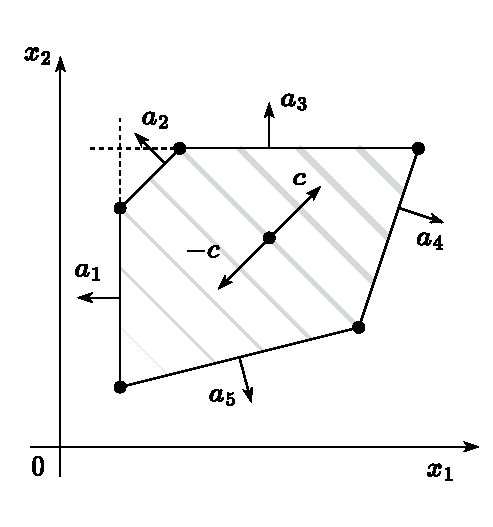
\includegraphics[keepaspectratio]{LP.pdf}}
\end{center}

В общем случае все задачи с линейной целевой функцией и линейными
функциональными ограничениями можно считать задачами линейного
программирования. Однако существует несколько стандартных формулировок.
\[
\tag{LP.Basic}
\begin{split}
&\min_{x \in \mathbb{R}^n} c^{\top}x \\
\text{s.t. } & Ax \leq b\\
\end{split}
\] для некоторых векторов \(c \in \mathbb{R}^n\), \(b \in \mathbb{R}^m\)
и матрицы \(A \in \mathbb{R}^{m \times n}\), где неравенства ---
покомпонентные. Мы будем часто использовать эту формулировку для
построения интуиции.

Широко используется \textbf{стандартная форма} записи задачи линейного
программирования. Пусть заданы векторы \(c \in \mathbb{R}^n\),
\(b \in \mathbb{R}^m\) и матрица \(A \in \mathbb{R}^{m \times n}\). \[
\tag{LP.Standard}
\begin{split}
&\min_{x \in \mathbb{R}^n} c^{\top}x \\
\text{s.t. } & Ax = b\\
& x_i \geq 0, \; i = 1,\dots, n
\end{split}
\]

\subsection{Задача о
диете}\label{ux437ux430ux434ux430ux447ux430-ux43e-ux434ux438ux435ux442ux435}

\begin{center}
\pandocbounded{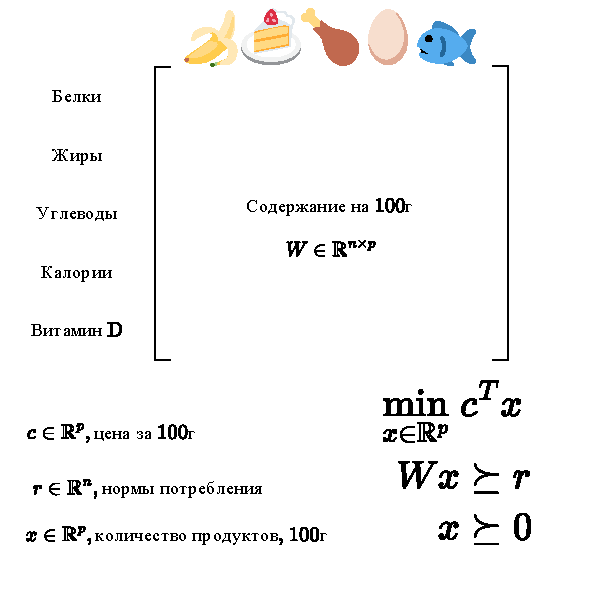
\includegraphics[keepaspectratio]{diet_LP_ru.pdf}}
\end{center}

Представьте, что вам нужно составить план диеты из некоторых продуктов:
бананы, пироги, курица, яйца, рыба. Каждый из продуктов имеет свой
вектор питательных веществ. Таким образом, все питательные вещества
можно представить в виде матрицы \(W\).

Предположим, что у нас есть вектор требований для каждого питательного
вещества \(r \in \mathbb{R}^n\). Нам нужно найти самую дешёвую диету,
которая удовлетворяет всем требованиям:

\[
\begin{split}
&\min_{x \in \mathbb{R}^p} c^{\top}x \\
\text{s.t. } & Wx \succeq r\\
& x_i \geq 0, \; i = 1,\dots, p
\end{split}
\]

\href{https://colab.research.google.com/github/MerkulovDaniil/optim/blob/master/assets/Notebooks/LP.ipynb\#scrollTo=fpT9Ywy5obfu}{\faPython Open
In Colab}

\subsection{Минимизация выпуклой функции как задача линейного
программирования}\label{ux43cux438ux43dux438ux43cux438ux437ux430ux446ux438ux44f-ux432ux44bux43fux443ux43aux43bux43eux439-ux444ux443ux43dux43aux446ux438ux438-ux43aux430ux43a-ux437ux430ux434ux430ux447ux430-ux43bux438ux43dux435ux439ux43dux43eux433ux43e-ux43fux440ux43eux433ux440ux430ux43cux43cux438ux440ux43eux432ux430ux43dux438ux44f}

\begin{figure}[H]

{\centering 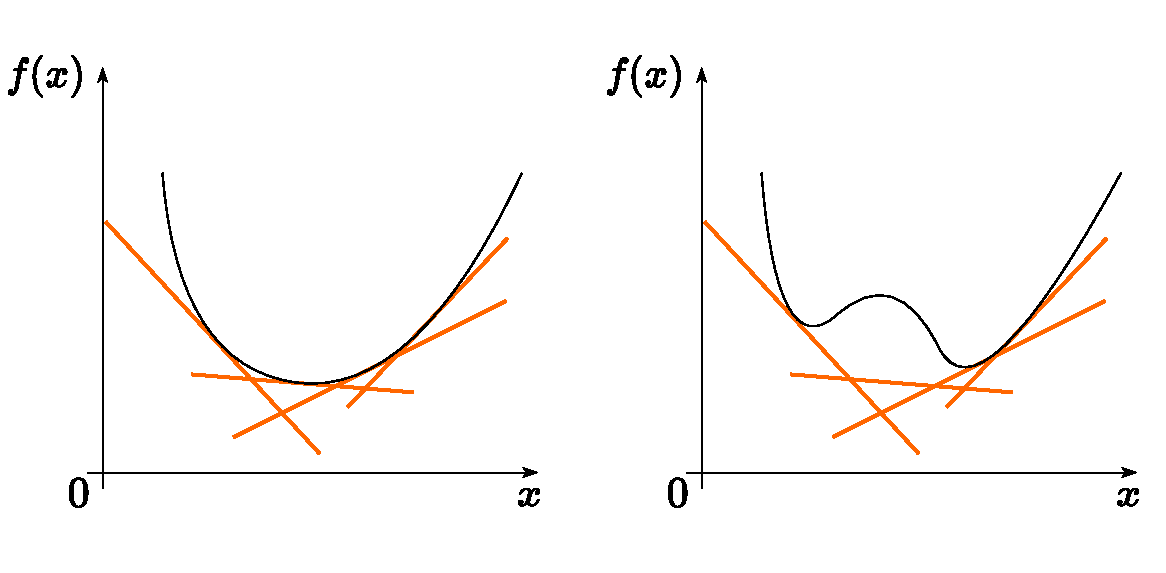
\includegraphics[width=0.75\linewidth,height=\textheight,keepaspectratio]{convex_via_LP.pdf}

}

\caption{Как задача линейного программирования может помочь с общей
задачей выпуклой оптимизации}

\end{figure}%

\begin{itemize}
\tightlist
\item
  Функция выпукла, если она может быть представлена как поточечный
  максимум линейных функций.
\item
  В пространствах большой размерности аппроксимация может потребовать
  огромного количества функций.
\item
  Существуют более эффективные солверы для выпуклой оптимизации (не
  сводящиеся к LP).
\end{itemize}

\subsection{\texorpdfstring{\href{https://jckantor.github.io/ND-Pyomo-Cookbook/notebooks/03.01-Transportation-Networks.html}{Транспортная
задача}}{Транспортная задача}}\label{ux442ux440ux430ux43dux441ux43fux43eux440ux442ux43dux430ux44f-ux437ux430ux434ux430ux447ux430}

Типичная транспортная задача заключается в распределении товара от
производителей к потребителям. Цель состоит в минимизации общих затрат
на транспортировку при соблюдении ограничений на количество товара на
каждом источнике и удовлетворении требований к спросу на каждом пункте
назначения.

\begin{figure}[H]

{\centering \pandocbounded{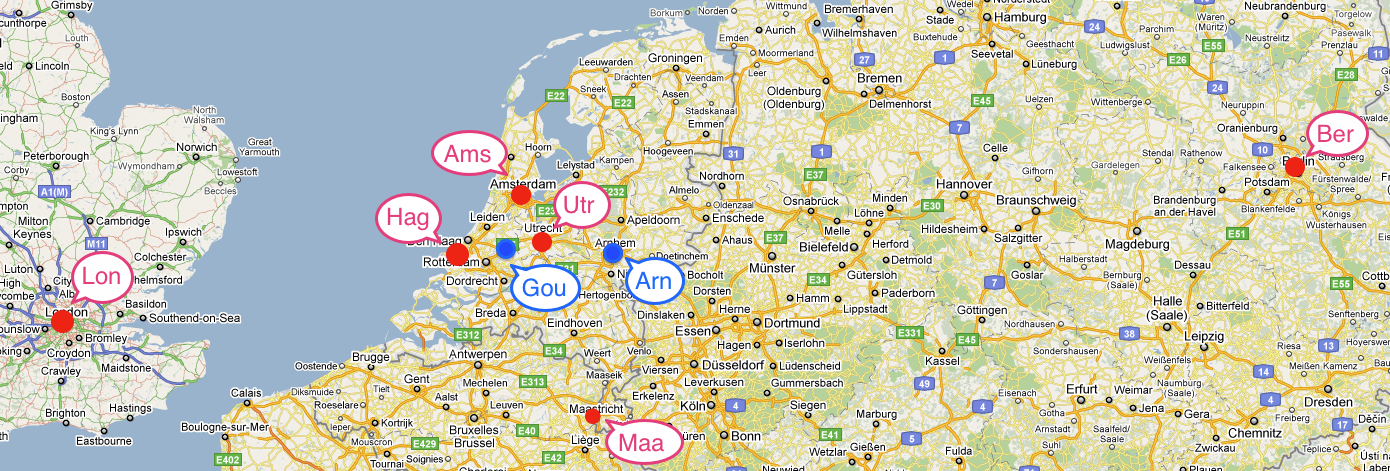
\includegraphics[keepaspectratio]{LP_west_europe.png}}

}

\caption{Карта Западной Европы.
\href{https://colab.research.google.com/github/MerkulovDaniil/optim/blob/master/assets/Notebooks/LP_transport.ipynb}{\faPython Open
In Colab}}

\end{figure}%

\begin{longtable}[]{@{}
  >{\centering\arraybackslash}p{(\linewidth - 6\tabcolsep) * \real{0.4211}}
  >{\centering\arraybackslash}p{(\linewidth - 6\tabcolsep) * \real{0.2105}}
  >{\centering\arraybackslash}p{(\linewidth - 6\tabcolsep) * \real{0.2105}}
  >{\centering\arraybackslash}p{(\linewidth - 6\tabcolsep) * \real{0.1579}}@{}}
\toprule\noalign{}
\begin{minipage}[b]{\linewidth}\centering
Пункт назначения / Источник
\end{minipage} & \begin{minipage}[b]{\linewidth}\centering
Арнем {[}\faEuroSign/тонна{]}
\end{minipage} & \begin{minipage}[b]{\linewidth}\centering
Гауда {[}\faEuroSign/тонна{]}
\end{minipage} & \begin{minipage}[b]{\linewidth}\centering
Спрос {[}тонн{]}
\end{minipage} \\
\midrule\noalign{}
\endhead
\bottomrule\noalign{}
\endlastfoot
Лондон & n/a & 2.5 & 125 \\
Берлин & 2.5 & n/a & 175 \\
Маастрихт & 1.6 & 2.0 & 225 \\
Амстердам & 1.4 & 1.0 & 250 \\
Утрехт & 0.8 & 1.0 & 225 \\
Гаага & 1.4 & 0.8 & 200 \\
\textbf{Макс. производство {[}тонн{]}} & 550 & 700 & \\
\end{longtable}

\vspace{-0.8cm}

\[
\text{Минимизировать:}\quad \text{Стоимость} = \sum_{c \in \text{Пункты назначения}}\sum_{s \in \text{Источники}} T[c,s] x[c,s]
\]

\[
\sum_{c \in \text{Пункты назначения}} x[c,s] \leq \text{Поставка}[s] \qquad \forall s \in \text{Источники}
\]

\[
\sum_{s\in \text{Источники}} x[c,s] = \text{Спрос}[c] \qquad \forall c \in \text{Пункты назначения}
\]

Задачу можно представить в виде следующего графа:

\begin{figure}[H]

{\centering \pandocbounded{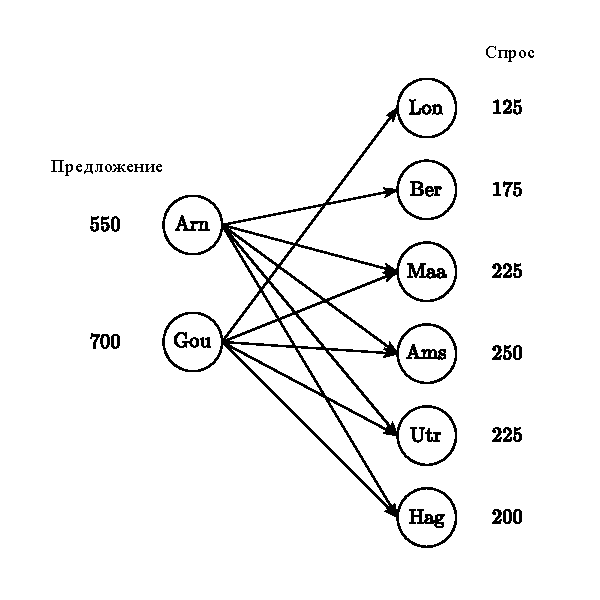
\includegraphics[keepaspectratio]{LP_transport_graph_ru.pdf}}

}

\caption{Граф, связанный с задачей}

\end{figure}%

\section{Как получить задачу линейного
программирования?}\label{ux43aux430ux43a-ux43fux43eux43bux443ux447ux438ux442ux44c-ux437ux430ux434ux430ux447ux443-ux43bux438ux43dux435ux439ux43dux43eux433ux43e-ux43fux440ux43eux433ux440ux430ux43cux43cux438ux440ux43eux432ux430ux43dux438ux44f}

\subsection{Основные
преобразования}\label{ux43eux441ux43dux43eux432ux43dux44bux435-ux43fux440ux435ux43eux431ux440ux430ux437ux43eux432ux430ux43dux438ux44f}

\begin{itemize}
\item
  Максимум-минимум \[
    \begin{split}
    &\min_{x \in \mathbb{R}^n} c^{\top}x \\
    \text{s.t. } & Ax \leq b\\
    \end{split} \quad \leftrightarrow \quad
    \begin{split}
    &\max_{x \in \mathbb{R}^n} -c^{\top}x \\
    \text{s.t. } & Ax \leq b\\
    \end{split} 
    \]
\item
  Равенство к неравенству \[
    Ax = b \leftrightarrow 
    \begin{cases}
    Ax \leq  b\\
    Ax \geq b
    \end{cases}
    \]
\item
  Неравенство к равенству, увеличивая размерность задачи на \(m\). \[
    Ax \leq b \leftrightarrow 
    \begin{cases}
    Ax + z =  b\\
    z \geq 0
    \end{cases}
    \]
\item
  Неотрицательные переменные \[
    x \leftrightarrow 
    \begin{cases}
    x = x_+ - x_-\\
    x_+ \geq 0 \\
    x_- \geq 0
    \end{cases}
    \]
\end{itemize}

\subsection{Задача аппроксимации
Чебышева}\label{ux437ux430ux434ux430ux447ux430-ux430ux43fux43fux440ux43eux43aux441ux438ux43cux430ux446ux438ux438-ux447ux435ux431ux44bux448ux435ux432ux430}

\[
\min_{x \in \mathbb{R}^n} \|Ax - b\|_\infty \leftrightarrow \min_{x \in \mathbb{R}^n} \max_{i} |a_i^T x - b_i|
\]

Можно записать эквивалентную задачу линейного программирования с заменой
максимальной координаты вектора:

\[
\begin{split}
&\min_{t \in \mathbb{R}, x \in \mathbb{R}^n} t \\
\text{s.t. } & a_i^T x - b_i \leq t, \; i = 1,\dots, m\\
& -a_i^T x + b_i \leq t, \; i = 1,\dots, m
\end{split}
\]

\subsection{\texorpdfstring{Задача
\(\ell_1\)-аппроксимации}{Задача \textbackslash ell\_1-аппроксимации}}\label{ux437ux430ux434ux430ux447ux430-ell_1-ux430ux43fux43fux440ux43eux43aux441ux438ux43cux430ux446ux438ux438}

\[
\min_{x \in \mathbb{R}^n} \|Ax - b\|_1 \leftrightarrow \min_{x \in \mathbb{R}^n} \sum_{i=1}^m |a_i^T x - b_i|
\]

Можно записать эквивалентную задачу линейного программирования с заменой
суммы координат вектора:

\[
\begin{split}
&\min_{t \in \mathbb{R}^m, x \in \mathbb{R}^n} \mathbf{1}^T t \\
\text{s.t. } & a_i^T x - b_i \leq t_i, \; i = 1,\dots, m\\
& -a_i^T x + b_i \leq t_i, \; i = 1,\dots, m
\end{split}
\]

\subsection[Задача смешивания: от нелинейных ограничений к ЛП
]{\texorpdfstring{Задача смешивания: от нелинейных ограничений к ЛП
\footnote{\href{https://jckantor.github.io/ND-Pyomo-Cookbook/notebooks/02.03-Linear-Blending-Problem.html}{Источник}}}{Задача смешивания: от нелинейных ограничений к ЛП }}\label{ux437ux430ux434ux430ux447ux430-ux441ux43cux435ux448ux438ux432ux430ux43dux438ux44f-ux43eux442-ux43dux435ux43bux438ux43dux435ux439ux43dux44bux445-ux43eux433ux440ux430ux43dux438ux447ux435ux43dux438ux439-ux43a-ux43bux43f}

Производственное предприятие получает заказ на 100 литров раствора с
определённой концентрацией (например, 4\% сахарного раствора). На складе
есть:

\begin{longtable}[]{@{}lcc@{}}
\toprule\noalign{}
Компонент & Сахар (\%) & Стоимость (\$/л) \\
\midrule\noalign{}
\endhead
\bottomrule\noalign{}
\endlastfoot
\textbf{Концентрат A (Добрый кола)} & 10.6 & 1.25 \\
\textbf{Концентрат B (Север кола)} & 4.5 & 1.02 \\
\textbf{Вода (Псыж)} & 0.0 & 0.62 \\
\end{longtable}

\textbf{Цель}: Найти смесь с минимальной стоимостью, которая
удовлетворит заказ.

\subsubsection{Целевая
функция}\label{ux446ux435ux43bux435ux432ux430ux44f-ux444ux443ux43dux43aux446ux438ux44f}

Минимизировать стоимость: \[
\text{Cost} = \sum_{c \in C} x_c P_c
\] где \(x_c\) --- объём используемого компонента \(c\), и \(P_c\) ---
его цена.

\subsubsection{Ограничение на
объём}\label{ux43eux433ux440ux430ux43dux438ux447ux435ux43dux438ux435-ux43dux430-ux43eux431ux44aux451ux43c}

Убедитесь, что общий объём \(V\): \[
V = \sum_{c \in C} x_c
\]

\paragraph{Ограничение на
состав}\label{ux43eux433ux440ux430ux43dux438ux447ux435ux43dux438ux435-ux43dux430-ux441ux43eux441ux442ux430ux432}

Убедитесь, что содержание сахара --- 4\%: \[
\bar{A} = \frac{\sum_{c \in C} x_c A_c}{\sum_{c \in C} x_c}
\]

Линеаризованная версия: \[
0 = \sum_{c \in C} x_c (A_c - \bar{A})
\] Это можно решить с помощью линейного программирования.

\href{https://colab.research.google.com/github/MerkulovDaniil/optim/blob/master/assets/Notebooks/LP_blending.ipynb}{\faPython Код}

\section{Симплекс-метод}\label{ux441ux438ux43cux43fux43bux435ux43aux441-ux43cux435ux442ux43eux434}

\subsection{Геометрия
симплекс-метода}\label{ux433ux435ux43eux43cux435ux442ux440ux438ux44f-ux441ux438ux43cux43fux43bux435ux43aux441-ux43cux435ux442ux43eux434ux430}

\begin{center}
\pandocbounded{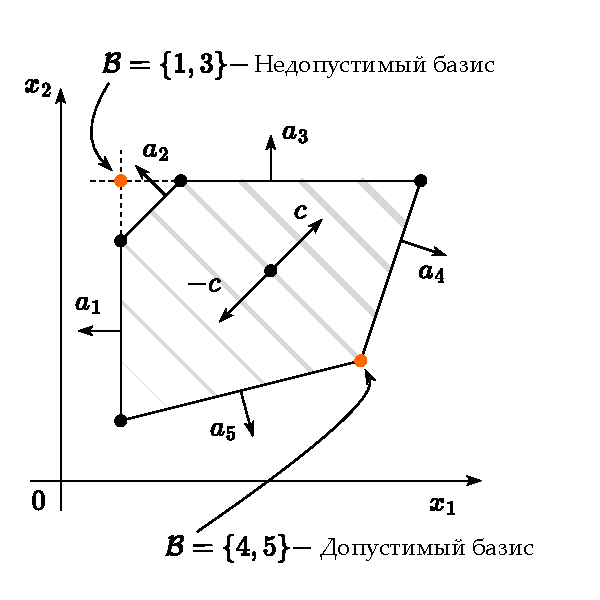
\includegraphics[keepaspectratio]{LP_basis_ru.pdf}}
\end{center}

Рассмотрим следующую простую формулировку задачи линейного
программирования:

\[
\tag{LP.Inequality}
\begin{split}
&\min_{x \in \mathbb{R}^n} c^{\top}x \\
\text{s.t. } & Ax \leq b
\end{split}
\]

\begin{itemize}
\tightlist
\item
  Определение: \textbf{базис} \(\mathcal{B}\) --- это подмножество \(n\)
  (целых) чисел между \(1\) и \(m\), такое что
  \(\text{rank} A_{\mathcal{B}} = n\).
\item
  Обратите внимание, что мы можем связать подматрицу \(A_{\mathcal{B}}\)
  и соответствующую правую часть \(b_{\mathcal{B}}\) с базисом
  \(\mathcal{B}\).
\item
  Также мы можем получить точку пересечения всех этих гиперплоскостей из
  базиса: \(x_{\mathcal{B}} = A^{-1}_{\mathcal{B}} b_{\mathcal{B}}\).
\item
  Если \(A x_{\mathcal{B}} \leq b\), то базис \(\mathcal{B}\) является
  \textbf{допустимым}.
\item
  Базис \(\mathcal{B}\) оптимален, если \(x_{\mathcal{B}}\) является
  решением задачи \(\text{LP.Inequality}\).
\item
  \(x_{\mathcal{B}}\) называют \textbf{базисной точкой} или базисным
  решением (иногда её тоже называют \textbf{базисом}).
\end{itemize}

\subsection{Если решение задачи линейного программирования существует,
то оно лежит в
вершине}\label{ux435ux441ux43bux438-ux440ux435ux448ux435ux43dux438ux435-ux437ux430ux434ux430ux447ux438-ux43bux438ux43dux435ux439ux43dux43eux433ux43e-ux43fux440ux43eux433ux440ux430ux43cux43cux438ux440ux43eux432ux430ux43dux438ux44f-ux441ux443ux449ux435ux441ux442ux432ux443ux435ux442-ux442ux43e-ux43eux43dux43e-ux43bux435ux436ux438ux442-ux432-ux432ux435ux440ux448ux438ux43dux435}

\begin{center}
\pandocbounded{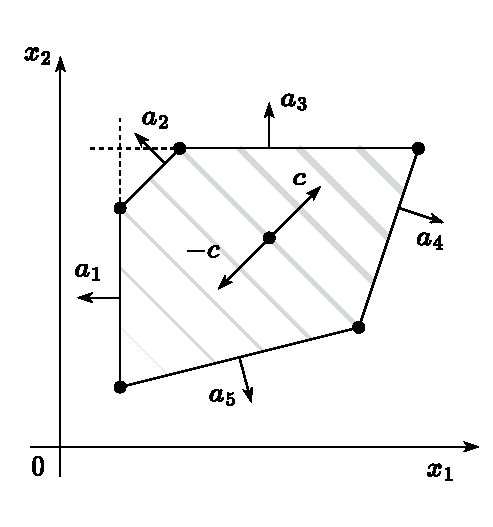
\includegraphics[keepaspectratio]{LP.pdf}}
\end{center}

\begin{tcolorbox}[enhanced jigsaw, coltitle=black, arc=.35mm, titlerule=0mm, colbacktitle=quarto-callout-color!10!white, bottomrule=.15mm, bottomtitle=1mm, colback=white, opacitybacktitle=0.6, breakable, opacityback=0, colframe=quarto-callout-color-frame, toprule=.15mm, toptitle=1mm, rightrule=.15mm, title=\textcolor{quarto-callout-color}{\faInfo}\hspace{0.5em}{Theorem}, leftrule=.75mm, left=2mm]

\begin{enumerate}
\def\labelenumi{\arabic{enumi}.}
\tightlist
\item
  Если задача линейного программирования в стандартной форме имеет
  непустое бюджетное множество, то существует по крайней мере одна
  допустимая базисная точка.
\item
  Если задача линейного программирования в стандартной форме имеет
  решения, то по крайней мере одно из таких решений является оптимальной
  базисной точкой.
\item
  Если задача линейного программирования в стандартной форме допустима и
  ограничена, то она имеет оптимальное решение.
\end{enumerate}

Для доказательства см. теорему 13.2 в
\href{https://fmin.xyz/assets/files/NumericalOptimization.pdf}{Numerical
Optimization by Jorge Nocedal and Stephen J. Wright}

\end{tcolorbox}

Верхнеуровневая идея симплекс-метода:

\begin{itemize}
\tightlist
\item
  Убедитесь, что вы находитесь в вершине.
\item
  Проверьте оптимальность.
\end{itemize}

\begin{itemize}
\tightlist
\item
  Если необходимо, перейдите к другой вершине (измените базис).
\item
  Повторяйте, пока не сойдётесь.
\end{itemize}

\subsection{Оптимальный
базис}\label{ux43eux43fux442ux438ux43cux430ux43bux44cux43dux44bux439-ux431ux430ux437ux438ux441}

\begin{center}
\pandocbounded{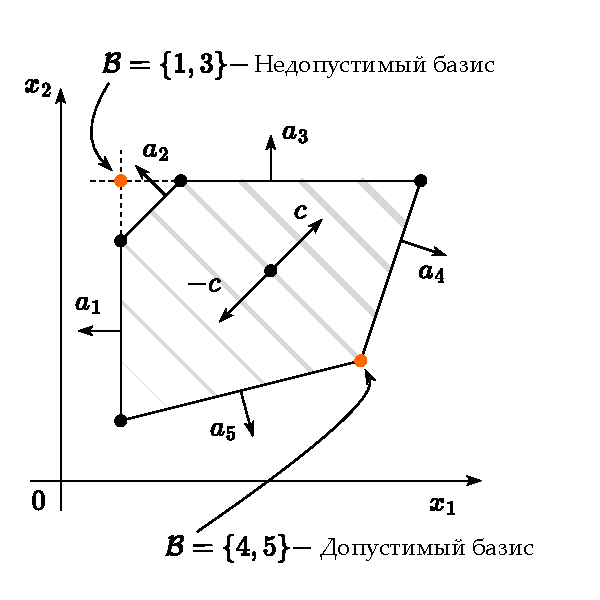
\includegraphics[keepaspectratio]{LP_basis_ru.pdf}}
\end{center}

Поскольку у нас есть базис, мы можем разложить наш целевой вектор \(c\)
в этом базисе и найти скалярные коэффициенты \(\lambda_{\mathcal{B}}\):
\[
\lambda^T_{\mathcal{B}} A_{\mathcal{B}} = c^T \leftrightarrow \lambda^T_{\mathcal{B}} = c^T A_{\mathcal{B}}^{-1}
\]

\begin{tcolorbox}[enhanced jigsaw, coltitle=black, arc=.35mm, titlerule=0mm, colbacktitle=quarto-callout-color!10!white, bottomrule=.15mm, bottomtitle=1mm, colback=white, opacitybacktitle=0.6, breakable, opacityback=0, colframe=quarto-callout-color-frame, toprule=.15mm, toptitle=1mm, rightrule=.15mm, title=\textcolor{quarto-callout-color}{\faInfo}\hspace{0.5em}{Theorem}, leftrule=.75mm, left=2mm]

Если все компоненты \(\lambda_{\mathcal{B}}\) неположительны и
\(\mathcal{B}\) допустим, то \(\mathcal{B}\) оптимален.

\end{tcolorbox}

\textbf{Доказательство} Предположим противное, то есть
\(\lambda_{\mathcal{B}} \leq 0\) и \(\mathcal{B}\) допустим, но не
оптимален. \[
\begin{split}
\exists x^*: Ax^* &\leq b, c^T x^* < c^T x_{\mathcal{B}} \\
A_{\mathcal{B}} x^* &\leq b_{\mathcal{B}}   \mid \lambda_{\mathcal{B}}^T \cdot  \leq 0 \\
\lambda_{\mathcal{B}}^T A_{\mathcal{B}} x^* &\geq \lambda_{\mathcal{B}}^T b_{\mathcal{B}} \\
c^T x^* & \geq \lambda_{\mathcal{B}}^T A_{\mathcal{B}} x_{\mathcal{B}} \\
c^T x^* & \geq c^T  x_{\mathcal{B}} \\
\end{split}
\]

\subsection{Изменение
базиса}\label{ux438ux437ux43cux435ux43dux435ux43dux438ux435-ux431ux430ux437ux438ux441ux430}

\begin{center}
\pandocbounded{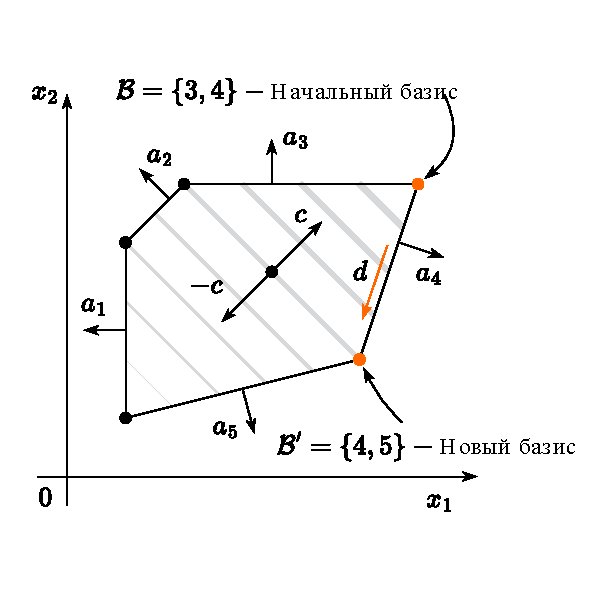
\includegraphics[keepaspectratio]{LP_change_ru.pdf}}
\end{center}

Предположим, что некоторые из коэффициентов \(\lambda_{\mathcal{B}}\)
положительны. В этом случае необходимо осуществить переход по ребру
многогранника к новой вершине, то есть произвести замену базиса.

\begin{itemize}
\item
  Предположим, что у нас есть базис \(\mathcal{B}\):
  \(\lambda^T_{\mathcal{B}} = c^T A_{\mathcal{B}}^{-1}\)
\item
  Предположим, что \(\lambda^k_{\mathcal{B}} > 0\). Мы хотим удалить
  \(k\) из базиса и сформировать новый: \[
     \begin{cases}
    A_{\mathcal{B} \textbackslash \{k\}} d = 0 \\
    a^T_k d = -1
    \end{cases} \qquad  c^Td   = \lambda^T_{\mathcal{B}} A_{\mathcal{B}} d  = \sum\limits_{i=1}^n \lambda^i_{\mathcal{B}}  (A_{\mathcal{B}} d)^i   = -\lambda^k_{\mathcal{B}} < 0 
    \]
\item
  Для всех \(j \notin \mathcal{B}\) рассчитаем размер шага проекции: \[
    \mu_j = \frac{b_j - a_j^T x_{\mathcal{B}}}{a_j^T d}
    \]
\item
  Определим новую вершину, которую мы добавим в новый базис: \[
    \begin{split}
    t = \text{arg}\min_j \{\mu_j \mid \mu_j > 0\} \\
    \mathcal{B}' = \mathcal{B}\textbackslash \{k\} \cup \{t\} \\ 
    x_{\mathcal{B'}} = x_{\mathcal{B}} + \mu_t d = A^{-1}_{\mathcal{B'}} b_{\mathcal{B'}}
    \end{split}
    \]
\item
  Обратите внимание, что изменение базиса приводит к уменьшению целевой
  функции:
  \(c^Tx_{\mathcal{B'}} = c^T(x_{\mathcal{B}} + \mu_t d) = c^Tx_{\mathcal{B}} + \mu_t c^Td\)
\end{itemize}

\subsection{Поиск начального допустимого
базиса}\label{ux43fux43eux438ux441ux43a-ux43dux430ux447ux430ux43bux44cux43dux43eux433ux43e-ux434ux43eux43fux443ux441ux442ux438ux43cux43eux433ux43e-ux431ux430ux437ux438ux441ux430}

Нам нужно решить следующую задачу:
\begin{equation}\phantomsection\label{eq-LP_ineq}{
\begin{split}
&\min_{x \in \mathbb{R}^n} c^{\top}x \\
\text{s.t. } & Ax \leq b
\end{split}
}\end{equation} Предложенный алгоритм требует начального допустимого
базиса.

Начнём с переформулировки задачи:
\begin{equation}\phantomsection\label{eq-LP_ineq_new}{
\begin{split}
&\min_{y \in \mathbb{R}^n, z \in \mathbb{R}^n} c^{\top}(y-z) \\
\text{s.t. } & Ay - Az \leq b \\ 
& y \geq 0, z \geq 0 \\ 
\end{split}
}\end{equation}

Зная решение задачи (\ref{eq-LP_ineq_new}), можно восстановить решение
задачи (\ref{eq-LP_ineq}), и наоборот.

\[
x = y-z \qquad \Leftrightarrow \qquad y_i = \max(x_i, 0), \quad z_i = \max(-x_i, 0)
\]

Теперь мы попытаемся сформулировать новую задачу линейного
программирования, решение которой будет допустимой базисной точкой для
Задачи~\ref{eq-LP_ineq_new}. Это означает, что мы сначала запускаем
симплекс-метод для задачи Phase-1, а затем запускаем задачу Phase-2 с
известным начальным решением. Обратите внимание, что допустимое базисное
решение для Phase-1 должно быть легко вычислимо.

\[
\tag{Фаза-2 (главная задача ЛП)}
\begin{split}
&\min_{y \in \mathbb{R}^n, z \in \mathbb{R}^n} c^{\top}(y-z) \\
\text{s.t. } & Ay - Az \leq b \\ 
& y \geq 0, z \geq 0 \\ 
\end{split}
\]

\[
\tag{Фаза-1}
\begin{split}
&\min_{\xi \in \mathbb{R}^m, y \in \mathbb{R}^n, z \in \mathbb{R}^n} \sum\limits_{i=1}^m \xi_i \\
\text{s.t. } & Ay - Az \leq b + \xi \\ 
& y \geq 0, z \geq 0, \xi \geq 0 \\ 
\end{split}
\]

\begin{itemize}
\item
  Если Фаза-2 (главная задача ЛП) имеет допустимое решение, то оптимум
  Фаза-1 равен нулю (т.е. все переменные \(\xi_i\) равны нулю).

  \textbf{Доказательство:} тривиальная проверка.
\item
  Если оптимум Фаза-1 равен нулю (т.е. все переменные \(\xi_i\) равны
  нулю), то мы получаем допустимый базис для Фаза-2.

  \textbf{Доказательство:} тривиальная проверка.
\end{itemize}

\begin{itemize}
\item
  Теперь мы знаем, что если мы можем решить задачу Фаза-1, то мы либо
  найдём начальную точку для симплекс-метода в исходном методе (если
  переменные \(\xi_i\) равны нулю), либо проверим, что исходная задача
  не имеет допустимого решения (если переменные \(\xi_i\) не равны
  нулю).
\item
  Но как решить задачу Фаза-1? Она имеет допустимое базисное решение
  (задача имеет \(2n + m\) переменных, и точка ниже гарантирует, что
  \(2n + m\) неравенств удовлетворяются как равенства (активны).)

  \[
    z = 0 \quad y = 0 \quad \xi_i = \max(0, -b_i)
    \]
\end{itemize}

\section{Сходимость
симплекс-метода}\label{ux441ux445ux43eux434ux438ux43cux43eux441ux442ux44c-ux441ux438ux43cux43fux43bux435ux43aux441-ux43cux435ux442ux43eux434ux430}

\subsection{Неограниченное бюджетное
множество}\label{ux43dux435ux43eux433ux440ux430ux43dux438ux447ux435ux43dux43dux43eux435-ux431ux44eux434ux436ux435ux442ux43dux43eux435-ux43cux43dux43eux436ux435ux441ux442ux432ux43e}

\begin{center}
\pandocbounded{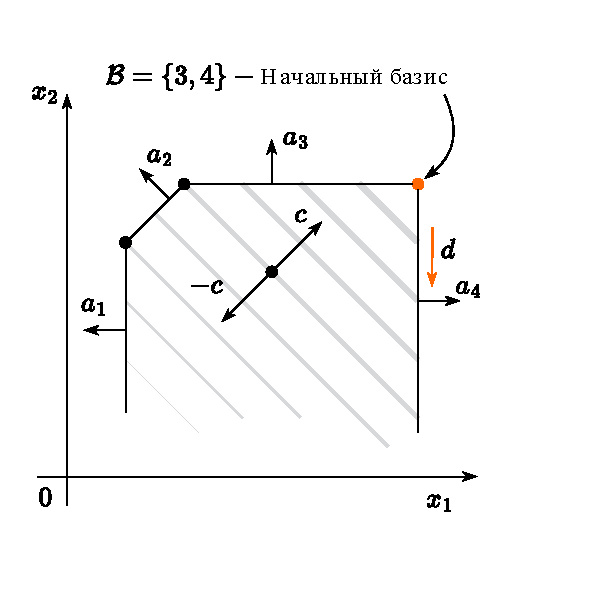
\includegraphics[keepaspectratio]{LP_unbounded_ru.pdf}}
\end{center}

В этом случае не найдётся ни одного положительного \(\mu_j\).

\subsection{Вырожденность
вершин}\label{ux432ux44bux440ux43eux436ux434ux435ux43dux43dux43eux441ux442ux44c-ux432ux435ux440ux448ux438ux43d}

\begin{center}
\pandocbounded{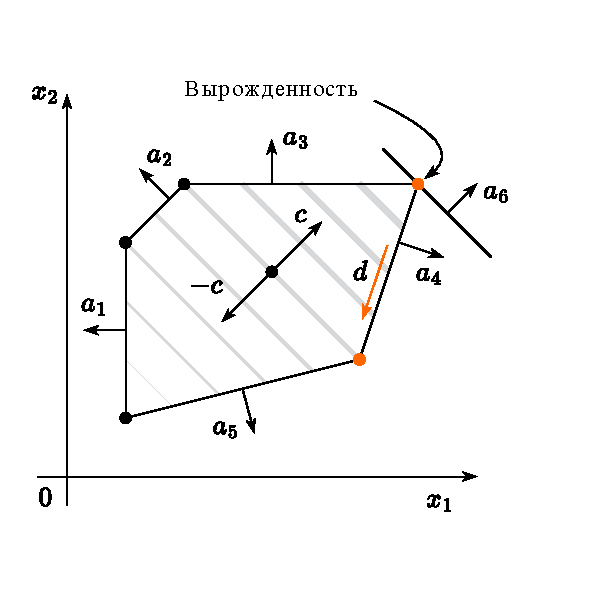
\includegraphics[keepaspectratio]{LP_degenerate_ru.pdf}}
\end{center}

Случаи вырожденности требуют особого рассмотрения. В отсутствие
вырожденности на каждой итерации гарантируется монотонное убывание
значения целевой функции.

\subsection{Экспоненциальная
сходимость}\label{ux44dux43aux441ux43fux43eux43dux435ux43dux446ux438ux430ux43bux44cux43dux430ux44f-ux441ux445ux43eux434ux438ux43cux43eux441ux442ux44c}

\pandocbounded{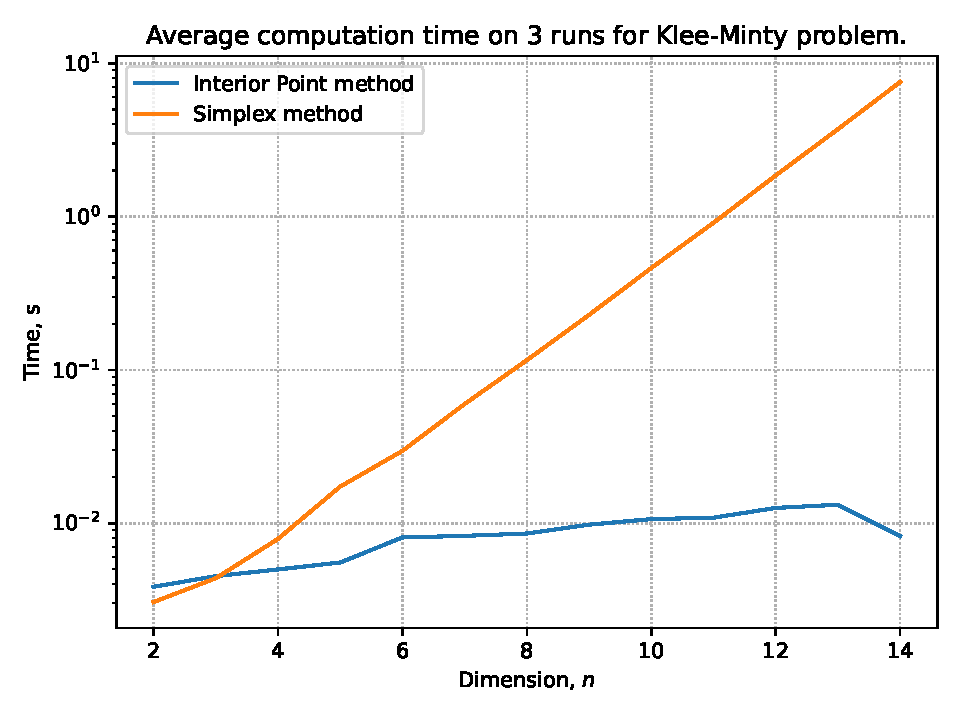
\includegraphics[keepaspectratio]{LP_IPM.pdf}}

\begin{itemize}
\tightlist
\item
  Много прикладных задач может быть сформулировано в виде задач
  линейного программирования.
\item
  Симплекс-метод прост в своей основе, но в худшем случае может работать
  экспоненциально долго.
\item
  Метод эллипсоидов Хачияна (1979) стал первым алгоритмом с доказанной
  полиномиальной сложностью для задач ЛП. Однако он обычно работает
  медленнее, чем симплекс-метод в реальных небольших задачах.
\item
  Основной прорыв --- метод Кармаркара (1984) для решения задач ЛП с
  использованием метода внутренней точки.
\item
  Методы внутренней точки являются последним словом в этой области. Тем
  не менее, для типовых задач ЛП качественные реализации симплекс-метода
  и методов внутренней точки показывают схожую производительность.
\end{itemize}

\subsection{\texorpdfstring{Пример
\href{https://en.wikipedia.org/wiki/Klee\%E2\%80\%93Minty_cube}{Klee
Minty}}{Пример Klee Minty}}\label{ux43fux440ux438ux43cux435ux440-klee-minty}

Так как число вершин конечно, сходимость алгоритма гарантирована (за
исключением вырожденных случаев, которые здесь не рассматриваются). Тем
не менее, сходимость может быть экспоненциально медленной из-за
потенциально большого числа вершин. Существует пример, в котором
симплекс-метод вынужден пройти через все вершины многогранника.

В следующей задаче симплекс-метод должен проверить \(2^n - 1\) вершин с
\(x_0 = 0\).

\[
\begin{split} 
& \max_{x \in \mathbb{R}^n} 2^{n-1}x_1 + 2^{n-2}x_2 + \dots + 2x_{n-1} + x_n \\
\text{s.t. } & x_1 \leq 5 \\
& 4x_1 + x_2 \leq 25 \\
& 8x_1 + 4x_2 + x_3 \leq 125 \\
& \ldots \\
& 2^n x_1 + 2^{n-1}x_2 + 2^{n-2}x_3 + \ldots + x_n \leq 5^n\\ 
& x \geq 0  
\end{split}
\]

\pandocbounded{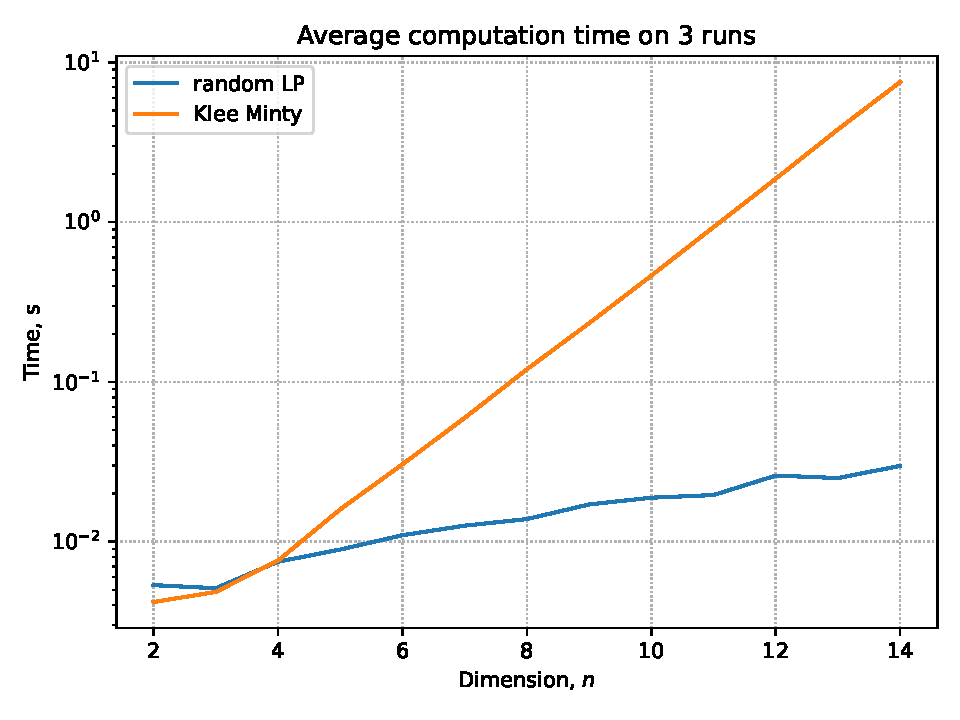
\includegraphics[keepaspectratio]{LP_KM.pdf}}

\section{Смешанное целочисленное программирование
(MIP)}\label{ux441ux43cux435ux448ux430ux43dux43dux43eux435-ux446ux435ux43bux43eux447ux438ux441ux43bux435ux43dux43dux43eux435-ux43fux440ux43eux433ux440ux430ux43cux43cux438ux440ux43eux432ux430ux43dux438ux435-mip}

\subsection{Сложность
MIP}\label{ux441ux43bux43eux436ux43dux43eux441ux442ux44c-mip}

Рассмотрим следующую задачу смешанного целочисленного программирования
(MIP): \begin{equation}\phantomsection\label{eq-mip}{
\begin{split}
z = 8x_1 + 11x_2 + 6x_3 + 4x_4 &\to \max_{x_1, x_2, x_3, x_4} \\
\text{s.t. }  5x_1+7x_2+4x_3+3x_4 &\leq 14 \\
x_i \in \{0,1\} \quad \forall i &
\end{split}
}\end{equation}

Упростим её до: \begin{equation}\phantomsection\label{eq-mip_lp_relax}{
\begin{split}
z = 8x_1 + 11x_2 + 6x_3 + 4x_4 &\to \max_{x_1, x_2, x_3, x_4} \\
\text{s.t. }  5x_1+7x_2+4x_3+3x_4 &\leq 14 \\
x_i \in [0,1] \quad \forall i &
\end{split}
}\end{equation}

Оптимальное решение \[
x_1=0, x_2=x_3=x_4=1, \text{ и } z=21.
\]

Оптимальное решение \[
x_1 = x_2 = 1, x_3 = 0.5, x_4 = 0, \text{ и } z = 22.
\]

\begin{itemize}
\tightlist
\item
  Округление \(x_3 = 0\): даёт \(z = 19\).
\item
  Округление \(x_3 = 1\): недопустимо.
\end{itemize}

\begin{tcolorbox}[enhanced jigsaw, coltitle=black, arc=.35mm, titlerule=0mm, colbacktitle=quarto-callout-important-color!10!white, bottomrule=.15mm, bottomtitle=1mm, colback=white, opacitybacktitle=0.6, breakable, opacityback=0, colframe=quarto-callout-important-color-frame, toprule=.15mm, toptitle=1mm, rightrule=.15mm, title=\textcolor{quarto-callout-important-color}{\faExclamation}\hspace{0.5em}{MIP намного сложнее, чем ЛП}, leftrule=.75mm, left=2mm]

\begin{itemize}
\tightlist
\item
  Наивное округление решения, полученного для ЛП-релаксации исходной
  задачи MIP, может привести к недопустимому или неоптимальному решению.
\item
  Общая задача MIP является NP-трудной задачей.
\item
  Однако, если матрица коэффициентов MIP является
  \href{https://en.wikipedia.org/wiki/Integer_programming}{\emph{полностью
  унимодулярной матрицей}}, то она может быть решена за полиномиальное
  время.
\end{itemize}

\end{tcolorbox}

\subsection{Непредсказуемая сложность
MIP}\label{ux43dux435ux43fux440ux435ux434ux441ux43aux430ux437ux443ux435ux43cux430ux44f-ux441ux43bux43eux436ux43dux43eux441ux442ux44c-mip}

\begin{itemize}
\tightlist
\item
  Трудно предсказать, что будет решено быстро, а что потребует много
  времени
\item
  \href{https://miplib.zib.de/index.html}{\faLink Датасет}
\item
  \href{https://colab.research.google.com/github/MerkulovDaniil/optim/blob/master/assets/Notebooks/miplib.ipynb}{\faPython Код}
\end{itemize}

\pandocbounded{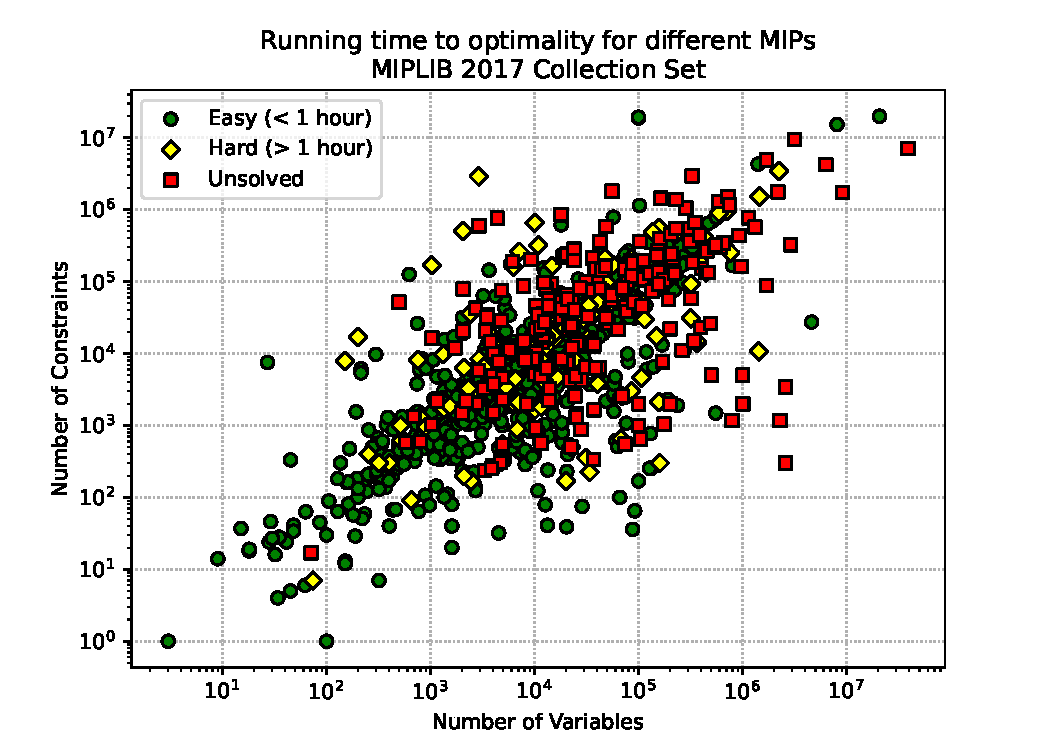
\includegraphics[keepaspectratio]{miplib.pdf}}

\subsection{Прогресс аппаратного vs программного
обеспечения}\label{ux43fux440ux43eux433ux440ux435ux441ux441-ux430ux43fux43fux430ux440ux430ux442ux43dux43eux433ux43e-vs-ux43fux440ux43eux433ux440ux430ux43cux43cux43dux43eux433ux43e-ux43eux431ux435ux441ux43fux435ux447ux435ux43dux438ux44f}

Что бы вы выбрали, если предположить, что вопрос поставлен корректно (вы
можете скомпилировать ПО для любого оборудования, и задача в обоих
случаях одна и та же)? Мы рассмотрим период с 1992 по 2023 год.

\begin{tcolorbox}[enhanced jigsaw, coltitle=black, arc=.35mm, titlerule=0mm, colbacktitle=quarto-callout-caution-color!10!white, bottomrule=.15mm, bottomtitle=1mm, colback=white, opacitybacktitle=0.6, breakable, opacityback=0, colframe=quarto-callout-caution-color-frame, toprule=.15mm, toptitle=1mm, rightrule=.15mm, title=\textcolor{quarto-callout-caution-color}{\faFire}\hspace{0.5em}{Аппаратное обеспечение}, leftrule=.75mm, left=2mm]

Решение MIP с использованием старого ПО на современном оборудовании

\end{tcolorbox}

\begin{tcolorbox}[enhanced jigsaw, coltitle=black, arc=.35mm, titlerule=0mm, colbacktitle=quarto-callout-caution-color!10!white, bottomrule=.15mm, bottomtitle=1mm, colback=white, opacitybacktitle=0.6, breakable, opacityback=0, colframe=quarto-callout-caution-color-frame, toprule=.15mm, toptitle=1mm, rightrule=.15mm, title=\textcolor{quarto-callout-caution-color}{\faFire}\hspace{0.5em}{Программное обеспечение}, leftrule=.75mm, left=2mm]

Решение MIP с использованием современного ПО на старом оборудовании

\end{tcolorbox}

\[
\approx 1.664.510\text{ x ускорение}
\] Закон Мура утверждает, что вычислительная мощность удваивается каждые
18 месяцев.

\[
\approx 2.349.000\text{ x ускорение}
\] Р. Бикси провёл масштабный эксперимент по сравнению
производительности всех версий CPLEX с 1992 по 2007 год и измерил общий
прогресс ПО (\(29 000\) раз), позже (в 2009 году) он стал одним из
основателей Gurobi Optimization, которое дало дополнительное
\(\approx 81\)
\href{https://www.gurobi.com/features/gurobi-optimizer-delivers-unmatched-performance/}{ускорение}
на MIP.

Оказывается, что если вам нужно решить MIP, лучше использовать старый
компьютер и современные методы, чем наоборот, самый новый компьютер и
методы начала 1990-х годов!\footnote{\href{https://www.math.uni-bielefeld.de/documenta/vol-ismp/25_bixby-robert.pdf}{R.
  Bixby report} \href{https://plato.asu.edu/talks/japan23.pdf}{Recent
  study}}

\subsection{Источники}\label{ux438ux441ux442ux43eux447ux43dux438ux43aux438}

\begin{itemize}
\tightlist
\item
  \href{https://www.math.cuhk.edu.hk/course_builder/1920/math4230/Lagrangeduality-example.pdf}{Теория
  оптимизации (MATH4230) курс @ CUHK, профессор Тейюн Цень}
\end{itemize}

\section{Задачи на
дом}\label{ux437ux430ux434ux430ux447ux438-ux43dux430-ux434ux43eux43c}

\begin{enumerate}
\def\labelenumi{\arabic{enumi}.}
\item
  \textbf{📱🎧💻 Производство чехлов.} {[}20 баллов{]} Lyzard Corp
  производит чехлы для следующих продуктов:

  \begin{itemize}
  \tightlist
  \item
    📱 телефоны
  \item
    🎧 наушники
  \item
    💻 ноутбуки
  \end{itemize}

  Производственные мощности компании таковы, что при полной загрузке
  производства выпуском чехлов для наушников, мы можем произвести 5000
  штук в день. Если мы посвятим всю производственную мощность чехлам для
  телефонов или ноутбуков, мы можем произвести 4000 или 2000 штук в
  день.

  Производственный цикл --- одна неделя (6 рабочих дней), и недельную
  продукцию необходимо разместить на складе до отгрузки. Хранение 1000
  чехлов для наушников (включая упаковку) занимает 30 кубических футов.
  Хранение 1000 чехлов для телефонов (включая упаковку) занимает 50
  кубических футов, а 1000 чехлов для ноутбуков --- 200 кубических
  футов. Доступный складской объём --- 1500 кубических футов. В силу
  коммерческих соглашений Lyzard Corp должна поставлять не менее 6000
  чехлов для наушников и 4000 чехлов для ноутбуков в неделю для усиления
  распространения продукта. Отдел маркетинга оценивает, что недельный
  спрос на чехлы для наушников, телефонов и ноутбуков не превышает
  15\,000, 12\,000 и 8000 единиц соответственно; следовательно, компания
  не хочет производить больше этих объёмов для указанных видов чехлов.

  Наконец, чистая прибыль на один чехол для наушников, чехол для
  телефона и чехол для ноутбука составляет 5, 7 и 12 долларов
  соответственно.

  Цель --- определить производственный график, который максимизирует
  общий чистый доход.

  \begin{enumerate}
  \def\labelenumii{\arabic{enumii}.}
  \item
    Напишите формулировку задачи линейного программирования для этой
    задачи. Используйте следующие переменные:

    \begin{itemize}
    \tightlist
    \item
      \(y_1\) = количество чехлов для наушников, произведенных за
      неделю,\\
    \item
      \(y_2\) = количество чехлов для телефонов, произведенных за
      неделю,\\
    \item
      \(y_3\) = количество чехлов для ноутбуков, произведенных за
      неделю.
    \end{itemize}
  \item
    Найдите решение задачи с помощью \href{http://www.pyomo.org}{PyOMO}

\begin{Shaded}
\begin{Highlighting}[]
\OperatorTok{!}\NormalTok{pip install pyomo}
\OperatorTok{!}\NormalTok{ sudo apt}\OperatorTok{{-}}\NormalTok{get install glpk}\OperatorTok{{-}}\NormalTok{utils }\OperatorTok{{-}{-}}\NormalTok{quiet  }\CommentTok{\# GLPK}
\OperatorTok{!}\NormalTok{ sudo apt}\OperatorTok{{-}}\NormalTok{get install coinor}\OperatorTok{{-}}\NormalTok{cbc }\OperatorTok{{-}{-}}\NormalTok{quiet  }\CommentTok{\# CoinOR}
\end{Highlighting}
\end{Shaded}
  \item
    Проведите анализ чувствительности. Какое ограничение можно ослабить,
    чтобы увеличить прибыль? Докажите это численно.
  \end{enumerate}
\item
  Докажите оптимальность решения {[}10 баллов{]}

  \[
   x = \left(\frac{7}{3} , 0, \frac{1}{3}\right)^T
   \]

  для следующей задачи линейного программирования:

  \[
   \begin{split}
   & 9x_1 + 3x_2 + 7x_3 \to \max\limits_{x \in \mathbb{R}^3 }\\
   \text{s.t. } & 2x_1 + x_2 + 3x_3 \leq 6 \\
   & 5x_1 + 4x_2 + x_3 \leq 12 \\
   & 3x_3 \leq 1,\\
   & x_1, x_2, x_3 \geq 0
   \end{split}
   \]

  но здесь нельзя использовать никакие численные алгоритмы.
\item
  {[}10 баллов{]} предположим, небольшая мастерская делает деревянные
  игрушки, где на каждый игрушечный поезд требуется одна заготовка
  древесины и 2 банки краски, а на каждую игрушечную лодку --- одна
  заготовка древесины и 1 банка краски. Прибыль с одного поезда
  составляет 30 долларов, с одной лодки --- 20 долларов. Имея запас 80
  заготовок древесины и 100 банок краски, какое количество каждой из
  игрушек следует произвести, чтобы максимизировать прибыль?

  \begin{enumerate}
  \def\labelenumii{\arabic{enumii}.}
  \tightlist
  \item
    Запишите оптимизационную задачу в стандартной форме, записывая все
    ограничения в виде неравенств.
  \item
    Нарисуйте допустимое множество и определите \(p^*\) и \(x^*\)
  \item
    Другая интерпретация множителей Лагранжа --- анализ чувствительности
    к изменению ограничений. Предположим, что мастерская нашла больше
    заготовок древесины; \(\lambda_k\) ассоциированная с ограничением на
    древесину, будет равна частной производной \(−p^*\) по отношению к
    тому, насколько больше древесины стало доступно. Предположим, что
    запас увеличился на одну заготовку древесины. Используйте
    \(\lambda^*\) для оценки того, насколько увеличится прибыль, без
    решения обновленной оптимизационной задачи. Как это согласуется с
    приведённой выше ценовой интерпретацией множителей
    Лагранжа?\href{https://tleise.people.amherst.edu/Math294Spring2017/TeXfiles/LagrangeDualityHW.pdf}{source}
  \end{enumerate}
\end{enumerate}




\end{document}
